\documentclass[aspectratio=169, 10pt]{beamer}

% --- Packages ---
\usepackage[utf8]{inputenc}
\usepackage[T1]{fontenc}
\usepackage{lmodern}
\usepackage{graphicx}

\usepackage{amsmath}
\usepackage{xcolor}
\usepackage{tikz}
\usetikzlibrary{positioning, arrows.meta, calc}

% Using default Computer Modern fonts for pdflatex compatibility

% --- Theme (Abstract Black) ---
\usetheme{default}
\usecolortheme{default}

% Dark monochromatic palette with neon accents
\definecolor{void}{RGB}{8, 8, 12}
\definecolor{abyss}{RGB}{16, 16, 22}
\definecolor{slate}{RGB}{28, 28, 36}
\definecolor{ash}{RGB}{55, 55, 68}
\definecolor{mist}{RGB}{160, 160, 175}
\definecolor{bone}{RGB}{220, 220, 228}
\definecolor{neonmint}{RGB}{0, 255, 180}
\definecolor{neonviolet}{RGB}{160, 80, 255}
\definecolor{neonpink}{RGB}{255, 60, 120}
\definecolor{neonamber}{RGB}{255, 190, 40}
\definecolor{neonice}{RGB}{80, 200, 255}

\setbeamercolor{normal text}{fg=bone, bg=void}
\setbeamercolor{structure}{fg=neonmint}
\setbeamercolor{palette primary}{bg=void, fg=bone}
\setbeamercolor{palette secondary}{bg=abyss, fg=bone}
\setbeamercolor{palette tertiary}{bg=slate, fg=bone}
\setbeamercolor{frametitle}{bg=, fg=bone}
\setbeamercolor{title}{fg=bone}
\setbeamercolor{subtitle}{fg=neonmint}
\setbeamercolor{author}{fg=mist}
\setbeamercolor{institute}{fg=ash}
\setbeamercolor{block title}{bg=slate, fg=neonmint}
\setbeamercolor{block body}{bg=abyss, fg=bone}
\setbeamercolor{block title alerted}{bg=slate, fg=neonpink}
\setbeamercolor{block body alerted}{bg=abyss, fg=bone}
\setbeamercolor{block title example}{bg=slate, fg=neonice}
\setbeamercolor{block body example}{bg=abyss, fg=bone}
\setbeamercolor{item}{fg=neonmint}
\setbeamercolor{subitem}{fg=mist}
\setbeamercolor{section in toc}{fg=bone}

% Remove ALL navigation and footers
\setbeamertemplate{navigation symbols}{}
\setbeamertemplate{footline}{}
\setbeamertemplate{headline}{}

% Minimal frame title
\setbeamertemplate{frametitle}{%
  \vspace{0.6em}%
  \noindent\hspace{0.5em}%
  {\large\bfseries\insertframetitle}%
  \vspace{-0.2em}%
  \par\noindent\hspace{0.5em}%
  \textcolor{neonmint}{\rule{2.5cm}{0.8pt}}%
  \vspace{0.3em}%
}

% Custom itemize markers
\setbeamertemplate{itemize item}{\color{neonmint}\tiny$\blacksquare$}
\setbeamertemplate{itemize subitem}{\color{ash}---}

% Blocks with left border accent
\setbeamertemplate{block begin}{%
  \vspace{0.3em}%
  \begin{beamercolorbox}[leftskip=0.4em, sep=0.5em, rounded=false]{block title}%
    \usebeamerfont{block title}\insertblocktitle%
  \end{beamercolorbox}%
  \begin{beamercolorbox}[leftskip=0.4em, sep=0.5em, rounded=false]{block body}%
}
\setbeamertemplate{block end}{\end{beamercolorbox}\vspace{0.3em}}

\setbeamertemplate{block alerted begin}{%
  \vspace{0.3em}%
  \begin{beamercolorbox}[leftskip=0.4em, sep=0.5em]{block title alerted}%
    \usebeamerfont{block title}\insertblocktitle%
  \end{beamercolorbox}%
  \begin{beamercolorbox}[leftskip=0.4em, sep=0.5em]{block body alerted}%
}
\setbeamertemplate{block alerted end}{\end{beamercolorbox}\vspace{0.3em}}

\setbeamertemplate{block example begin}{%
  \vspace{0.3em}%
  \begin{beamercolorbox}[leftskip=0.4em, sep=0.5em]{block title example}%
    \usebeamerfont{block title}\insertblocktitle%
  \end{beamercolorbox}%
  \begin{beamercolorbox}[leftskip=0.4em, sep=0.5em]{block body example}%
}
\setbeamertemplate{block example end}{\end{beamercolorbox}\vspace{0.3em}}

% --- Title Page Info ---
\title[Beyond the GPU]{Beyond the GPU}
\subtitle{A Microarchitectural Analysis of LLM Tool-Calling Kernels}
\author[Zhang, Rehman, Grewal]{Kunpeng Zhang \and Fazal Rehman \and TJ Grewal}
\institute[SFU]{CMPT 450}
\date{}

\begin{document}

% =================================================================
% SLIDE 1: TITLE
% =================================================================
\begin{frame}[plain]
  \begin{tikzpicture}[remember picture, overlay]
    % Abstract decorative elements
    \fill[neonmint, opacity=0.04] (current page.north west) ++(-1,-1) circle (8cm);
    \fill[neonviolet, opacity=0.03] (current page.south east) ++(2,2) circle (10cm);
    \draw[neonmint, opacity=0.15, line width=0.3pt] (current page.north west) ++(1.2,-3) -- ++(14,0);
    \draw[neonmint, opacity=0.08, line width=0.3pt] (current page.north west) ++(1.2,-3.3) -- ++(9,0);
  \end{tikzpicture}
  \vspace{2.5cm}
  \begin{flushleft}
    \hspace{1.5em}{\Huge\bfseries\textcolor{bone}{Beyond the GPU}}\\[0.4em]
    \hspace{1.5em}{\small\textcolor{neonmint}{A Microarchitectural Analysis of LLM Tool-Calling Kernels}}\\[1.8em]
    \hspace{1.5em}{\footnotesize\textcolor{mist}{Kunpeng Zhang \quad\textcolor{ash}{/}\quad Fazal Rehman \quad\textcolor{ash}{/}\quad TJ Grewal}}\\[0.3em]
    \hspace{1.5em}{\scriptsize\textcolor{ash}{CMPT 450}}\\[2em]
    \hspace{1.5em}{\scriptsize\textcolor{ash}{\textit{What happens when the CPU becomes the bottleneck for AI?}}}
  \end{flushleft}
\end{frame}

% =================================================================
% SLIDE 2: INTRODUCTION & MOTIVATION
% =================================================================
\begin{frame}{Introduction \& Motivation}
  \begin{tikzpicture}[remember picture, overlay]
    \fill[neonviolet, opacity=0.02] (current page.south west) ++(0,0) circle (6cm);
  \end{tikzpicture}
  \begin{columns}
    \begin{column}{0.55\textwidth}
      \begin{block}{The Paradigm Shift}
        LLMs are transitioning from \textbf{passive text generators} to \textbf{active, autonomous agents} utilized in complex engineering workflows.
      \end{block}
      \vspace{0.4em}
      \begin{block}{The Misplaced Focus}
        Historically, optimization efforts have overwhelmingly targeted the \textcolor{neonamber}{\textbf{GPU forward-pass}}, minimizing Time-To-First-Token (TTFT).
      \end{block}
    \end{column}
    \begin{column}{0.45\textwidth}
      \begin{alertblock}{The New Bottleneck}
        As tool-calling expands, the execution bottleneck shifts abruptly \textbf{from the hardware accelerator back to the host CPU}.
      \end{alertblock}
      \vspace{0.5em}
      \begin{center}
        \textcolor{neonmint}{\textbf{The CPU is the new frontier.}}
      \end{center}
    \end{column}
  \end{columns}
\end{frame}

% =================================================================
% SLIDE 3: ARCHITECTURAL DIVERGENCE
% =================================================================
\begin{frame}{Architectural Divergence}
  \begin{columns}
    \begin{column}{0.5\textwidth}
      \begin{block}{GPU Hostility}
        Agentic tool tasks behave more like traditional datacenter \textbf{Remote Procedure Calls (RPC)} than highly parallel machine learning kernels.
      \end{block}
      \vspace{0.3em}
      \begin{block}{Scalar by Nature}
        Operations like parsing JSON, traversing filesystems, and querying databases are \textbf{inherently scalar}.
      \end{block}
    \end{column}
    \begin{column}{0.5\textwidth}
      \begin{alertblock}{The Hardware Penalty}
        These tasks require deep recursive logic and complex memory pointer chasing, leading to:
        \begin{itemize}
          \item Massive \textbf{Last-Level Cache (LLC)} miss rates
          \item High \textbf{branch mispredictions}
          \item Frequent \textbf{pipeline stalls}
        \end{itemize}
      \end{alertblock}
      \vspace{0.3em}
      \begin{center}
        \textcolor{neonmint}{\textbf{Agent tools are fundamentally hostile to GPU architectures.}}
      \end{center}
    \end{column}
  \end{columns}
\end{frame}

% =================================================================
% SLIDE 4: CORE RESEARCH QUESTIONS
% =================================================================
\begin{frame}{Core Research Questions}
  \begin{tikzpicture}[remember picture, overlay]
    \fill[neonmint, opacity=0.02] (current page.north east) ++(-3,-2) circle (5cm);
  \end{tikzpicture}
  \vspace{0.5em}
  \begin{exampleblock}{RQ1 --- Quantification}
    What is the macro-level ``Agentic Tax'' (latency penalty) imposed strictly by the LLM orchestration framework?
  \end{exampleblock}
  \vspace{0.3em}
  \begin{exampleblock}{RQ2 --- Microarchitectural Profiling}
    How do specific tool classes map to their defining hardware bottlenecks during multi-step loops?
  \end{exampleblock}
  \vspace{0.3em}
  \begin{exampleblock}{RQ3 --- Optimization Viability}
    Do classical, kernel-level hardware optimizations effectively propagate to end-to-end system latency, or are they absorbed by the orchestration layer?
  \end{exampleblock}
\end{frame}

% =================================================================
% SLIDE 5: METHODOLOGY & SYSTEM ARCHITECTURE
% =================================================================
\begin{frame}{Methodology \& System Architecture}
  \begin{columns}
    \begin{column}{0.55\textwidth}
      \begin{block}{Decoupled Harness}
        Custom benchmarking suite that \textbf{strictly isolates} the Python/FastAPI orchestrator from compiled, native C++ execution kernels.
      \end{block}
      \vspace{0.3em}
      \begin{block}{The Model}
        \textbf{Qwen-2.5-7B-Instruct} running locally in FP16 with sampling disabled to guarantee \textbf{deterministic ReAct cycles}.
      \end{block}
    \end{column}
    \begin{column}{0.45\textwidth}
      \begin{block}{Cycle-Accurate Telemetry}
        Integrated the Linux PMU via \textbf{PAPI} to capture strictly scoped hardware events exclusively during CPU execution windows:
        \begin{itemize}
          \item Instructions Per Cycle (IPC)
          \item Branch Mispredictions
          \item L3 Cache Misses
          \item Total Cycles
        \end{itemize}
      \end{block}
    \end{column}
  \end{columns}
  \vspace{0.4em}
  \begin{center}
    \textcolor{mist}{\small Testbed: Intel Xeon Gold 6242R @ 3.10 GHz --- isolated, predictable cycle-to-latency.}
  \end{center}
\end{frame}

% =================================================================
% SLIDE 6: TOOL KERNELS & CONTROL BASELINE
% =================================================================
\begin{frame}{Tool Kernels \& Control Baseline}
  \begin{columns}
    \begin{column}{0.25\textwidth}
      \begin{block}{Compute-Bound}
        \textbf{AST Evaluator}\\[0.2em]
        {\small Nested math expressions stressing \textbf{branch prediction}.}
      \end{block}
    \end{column}
    \begin{column}{0.25\textwidth}
      \begin{block}{Memory-Bound}
        \textbf{SQLite Scan}\\[0.2em]
        {\small Forced full-table scans intentionally thrashing the \textbf{LLC}.}
      \end{block}
    \end{column}
    \begin{column}{0.25\textwidth}
      \begin{block}{I/O-Bound}
        \textbf{FS Walker}\\[0.2em]
        {\small Recursive traversal stressing \textbf{OS context switches}.}
      \end{block}
    \end{column}
    \begin{column}{0.25\textwidth}
      \begin{alertblock}{Control}
        \textbf{Direct Pipeline}\\[0.2em]
        {\small Static regex routing, \textbf{completely bypassing} the GPU \& LLM.}
      \end{alertblock}
    \end{column}
  \end{columns}
  \vspace{0.8em}
  \begin{center}
    \textcolor{neonmint}{\textbf{The ``Speed of Light'' control isolates the exact cost of orchestration.}}
  \end{center}
\end{frame}

% =================================================================
% SLIDE 7: KEY FINDING 1 - THE AGENTIC TAX
% =================================================================
\begin{frame}{Key Finding 1 --- The ``Agentic Tax''}
  \begin{columns}
    \begin{column}{0.55\textwidth}
      \begin{center}
        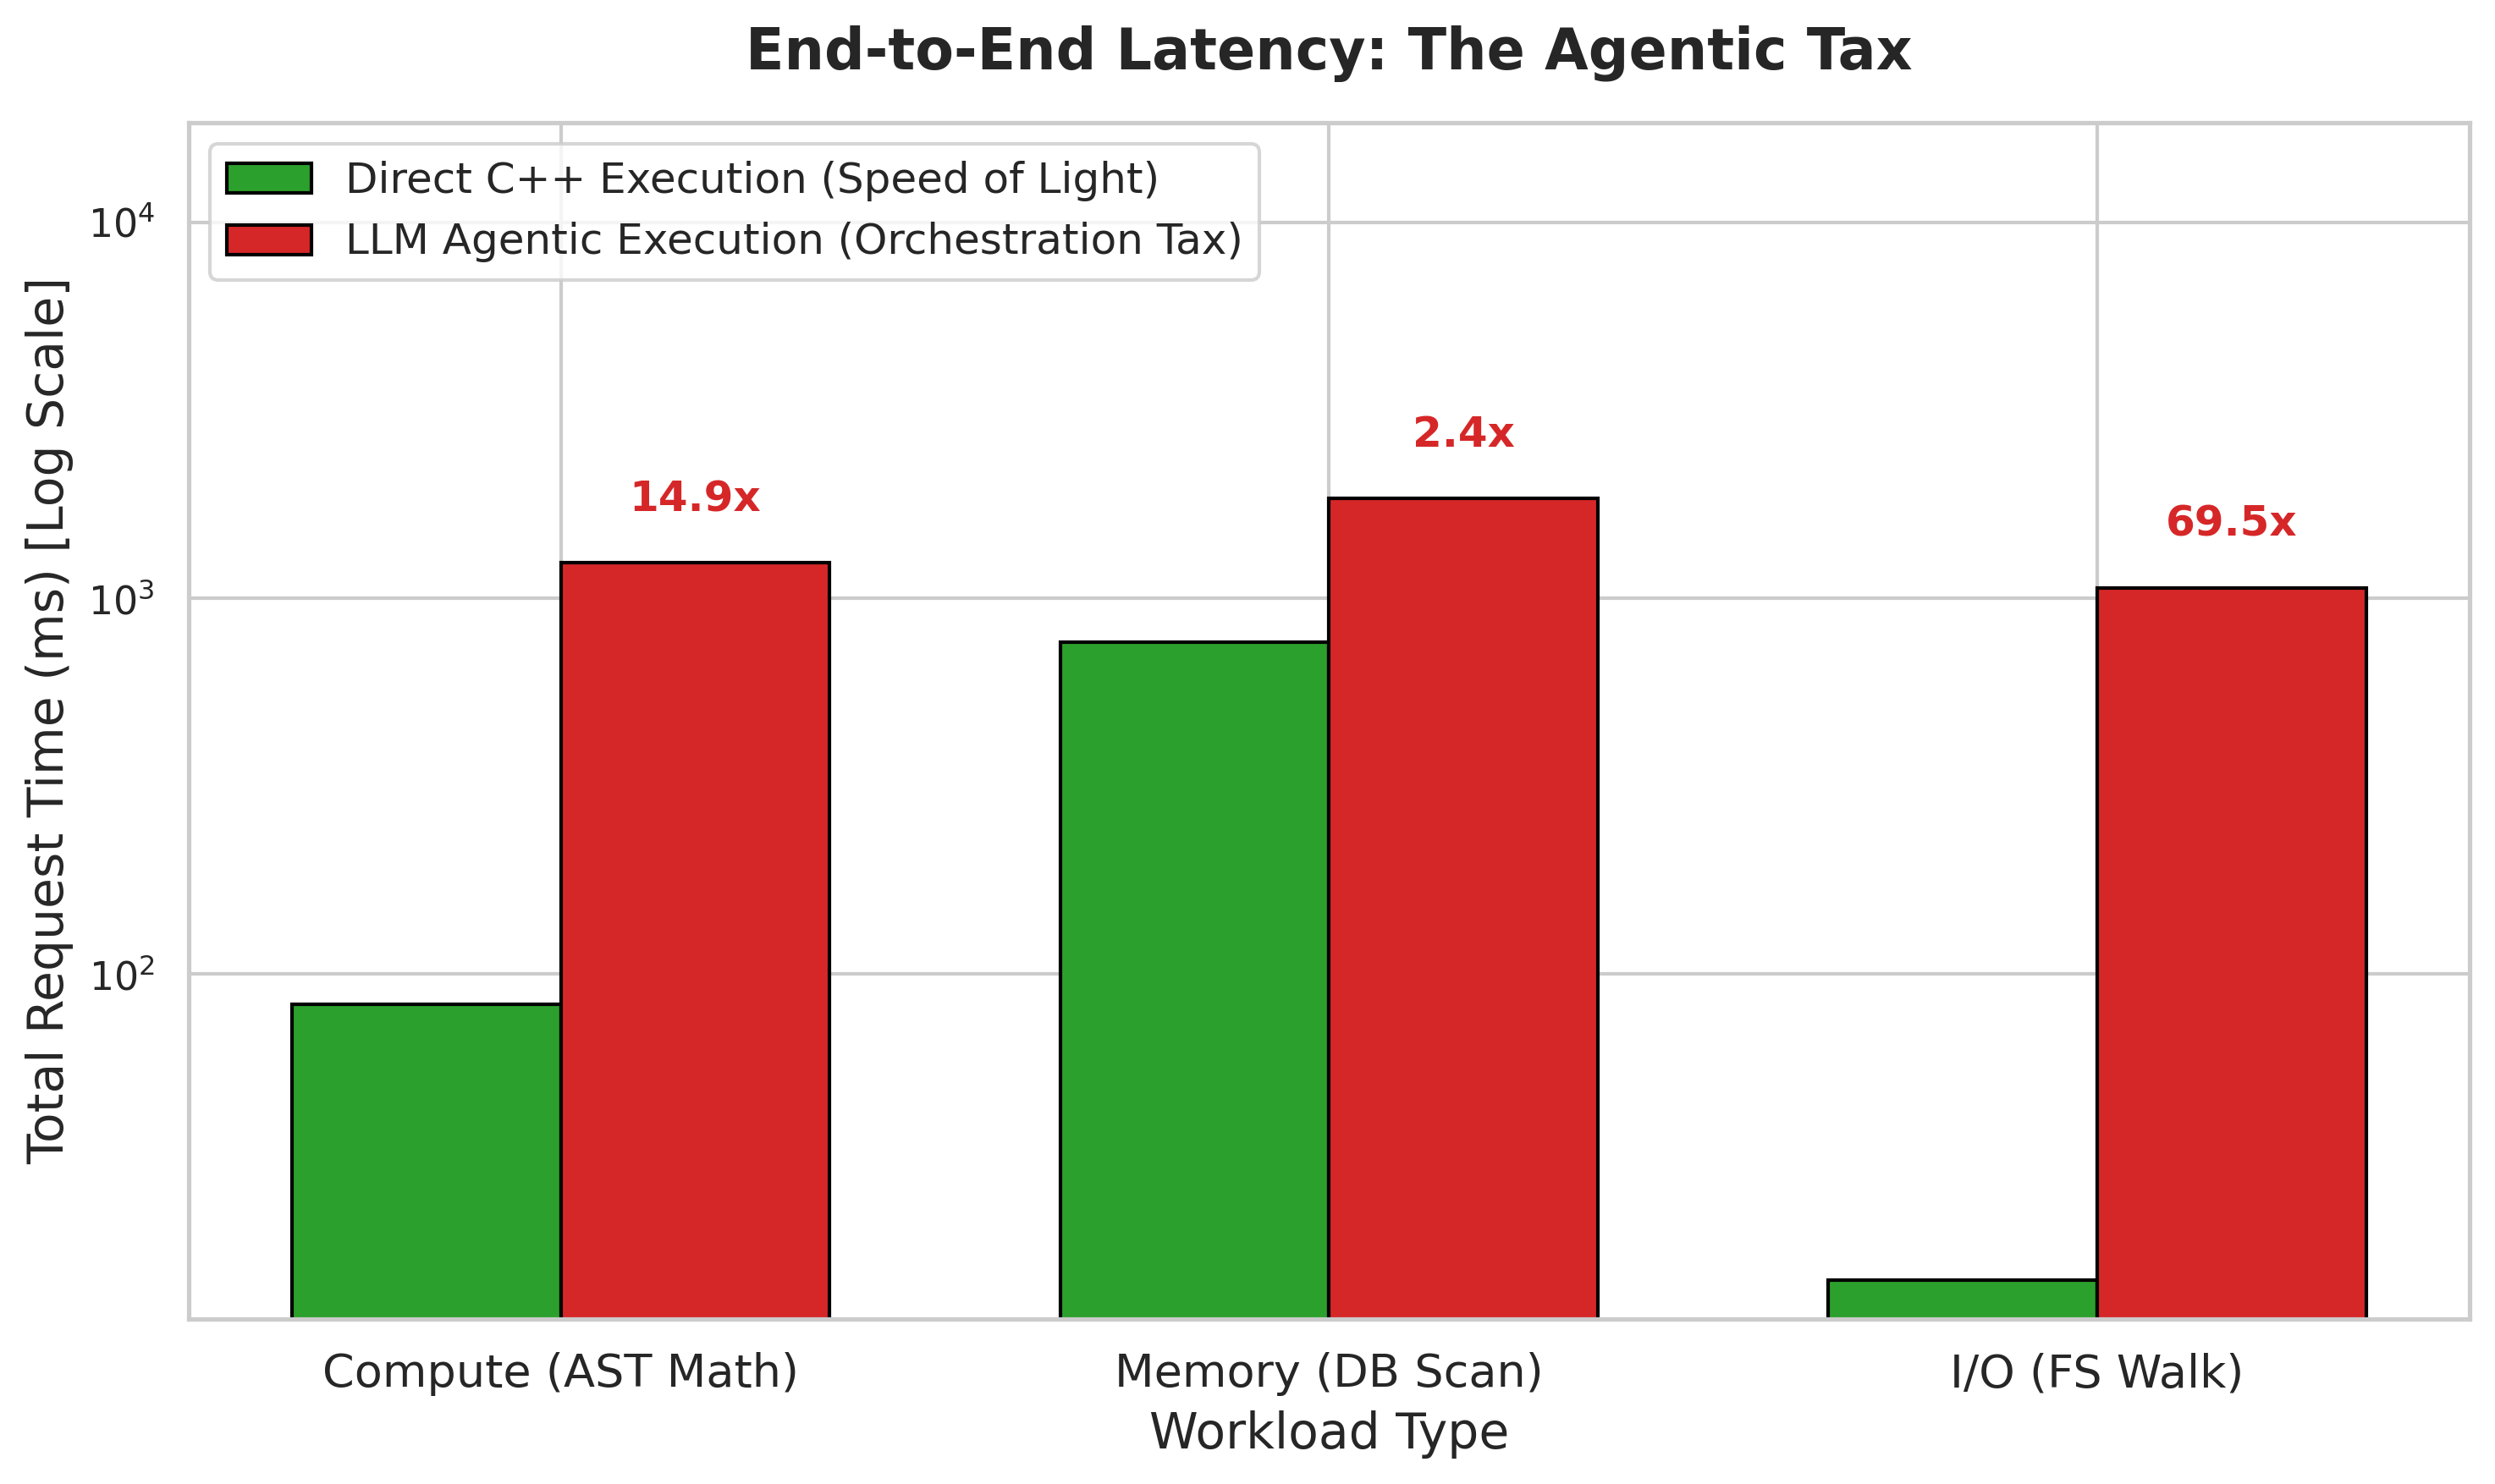
\includegraphics[width=\textwidth]{../results/ExpA_Agentic_Tax.png}
      \end{center}
      \vspace{-0.3em}
      {\scriptsize\textcolor{ash}{Figure 1: Log-scale latency --- Direct C++ vs.\ Full Agentic Loop.}}
    \end{column}
    \begin{column}{0.45\textwidth}
      \begin{itemize}
        \item \textcolor{neonpink}{\textbf{I/O Walk:}} Native $\sim$15\,ms $\rightarrow$ Agentic $\sim$1\,s\\
              \textbf{69.5$\times$} slowdown
        \item \textcolor{neonamber}{\textbf{AST Math:}} \textbf{14.9$\times$} penalty
        \item \textcolor{neonice}{\textbf{DB Scan:}} only \textbf{2.4$\times$} ($\sim$764\,ms native)
      \end{itemize}
      \vspace{0.3em}
      \begin{alertblock}{Amdahl's Law}
        The DB scan's 2.5 billion native cycles amortize the fixed framework cost. The tax is a \textbf{massive fixed cost}, not a proportional scalar.
      \end{alertblock}
    \end{column}
  \end{columns}
\end{frame}

% =================================================================
% SLIDE 8: KEY FINDING 2 - CONTEXT ACCUMULATION
% =================================================================
\begin{frame}{Key Finding 2 --- Context Accumulation (Multi-Step)}
  \begin{columns}
    \begin{column}{0.55\textwidth}
      \begin{center}
        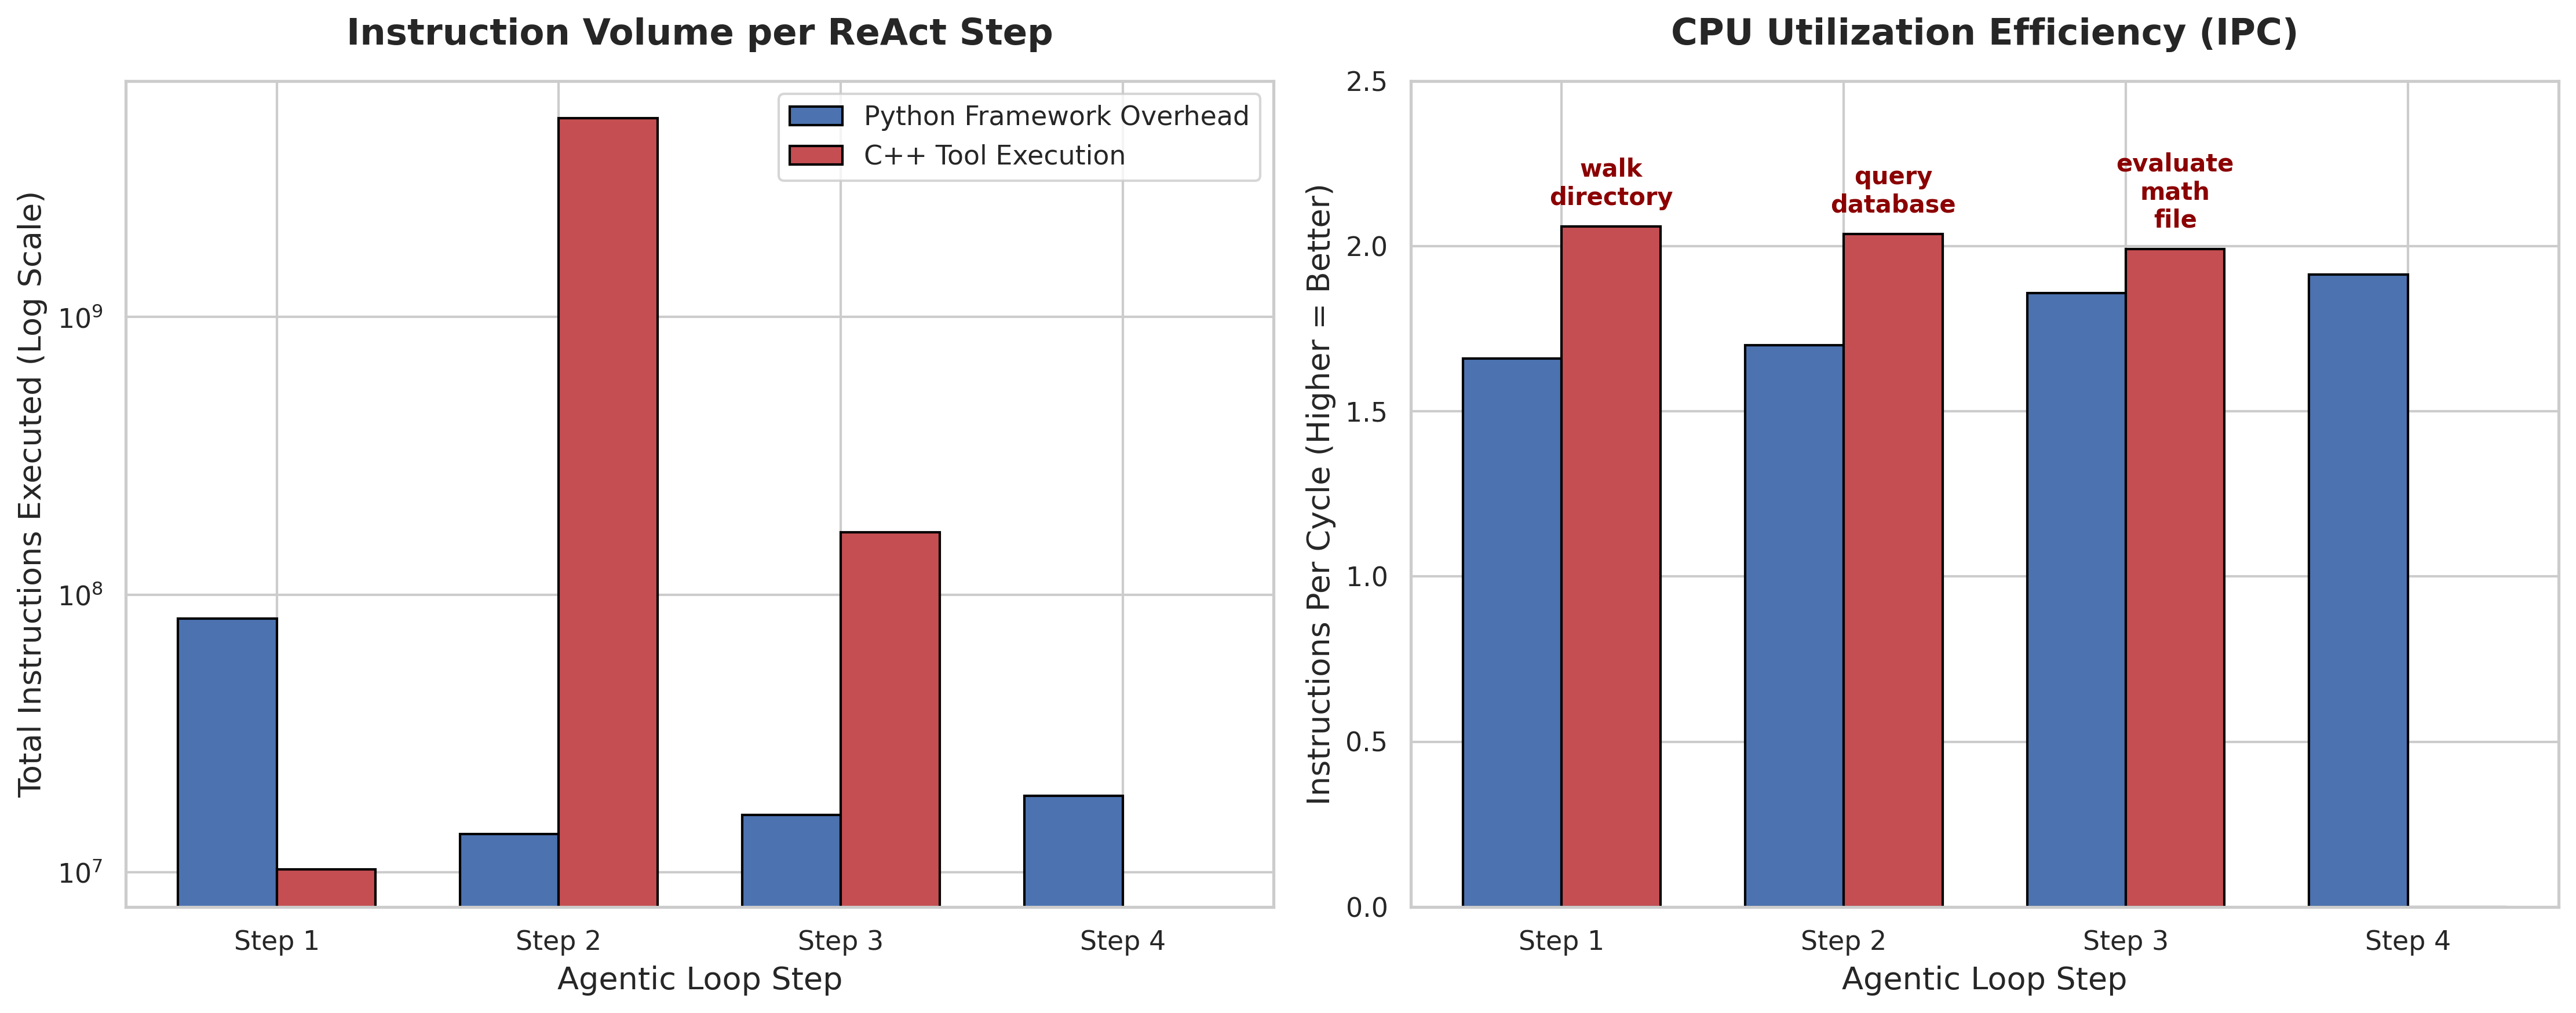
\includegraphics[width=\textwidth]{../results/ExpB_Multistep_Analysis.png}
      \end{center}
      \vspace{-0.3em}
      {\scriptsize\textcolor{ash}{Figure 2: Instruction volume \& IPC across a multi-step ReAct loop.}}
    \end{column}
    \begin{column}{0.45\textwidth}
      \begin{block}{The Cold Start Penalty}
        At Step~1, the framework executes $\sim$\textbf{82\,M instructions} simply to parse and load JSON schema definitions.
      \end{block}
      \vspace{0.3em}
      \begin{alertblock}{The Stateless Trap}
        Because the LLM is stateless, the framework's instruction volume \textbf{grows linearly} with each successive step, continuously re-serializing an expanding conversation history.
      \end{alertblock}
    \end{column}
  \end{columns}
\end{frame}

% =================================================================
% SLIDE 9: KEY FINDING 3 - THE MASKING EFFECT
% =================================================================
\begin{frame}{Key Finding 3 --- The Masking Effect}
  \begin{columns}
    \begin{column}{0.55\textwidth}
      \begin{center}
        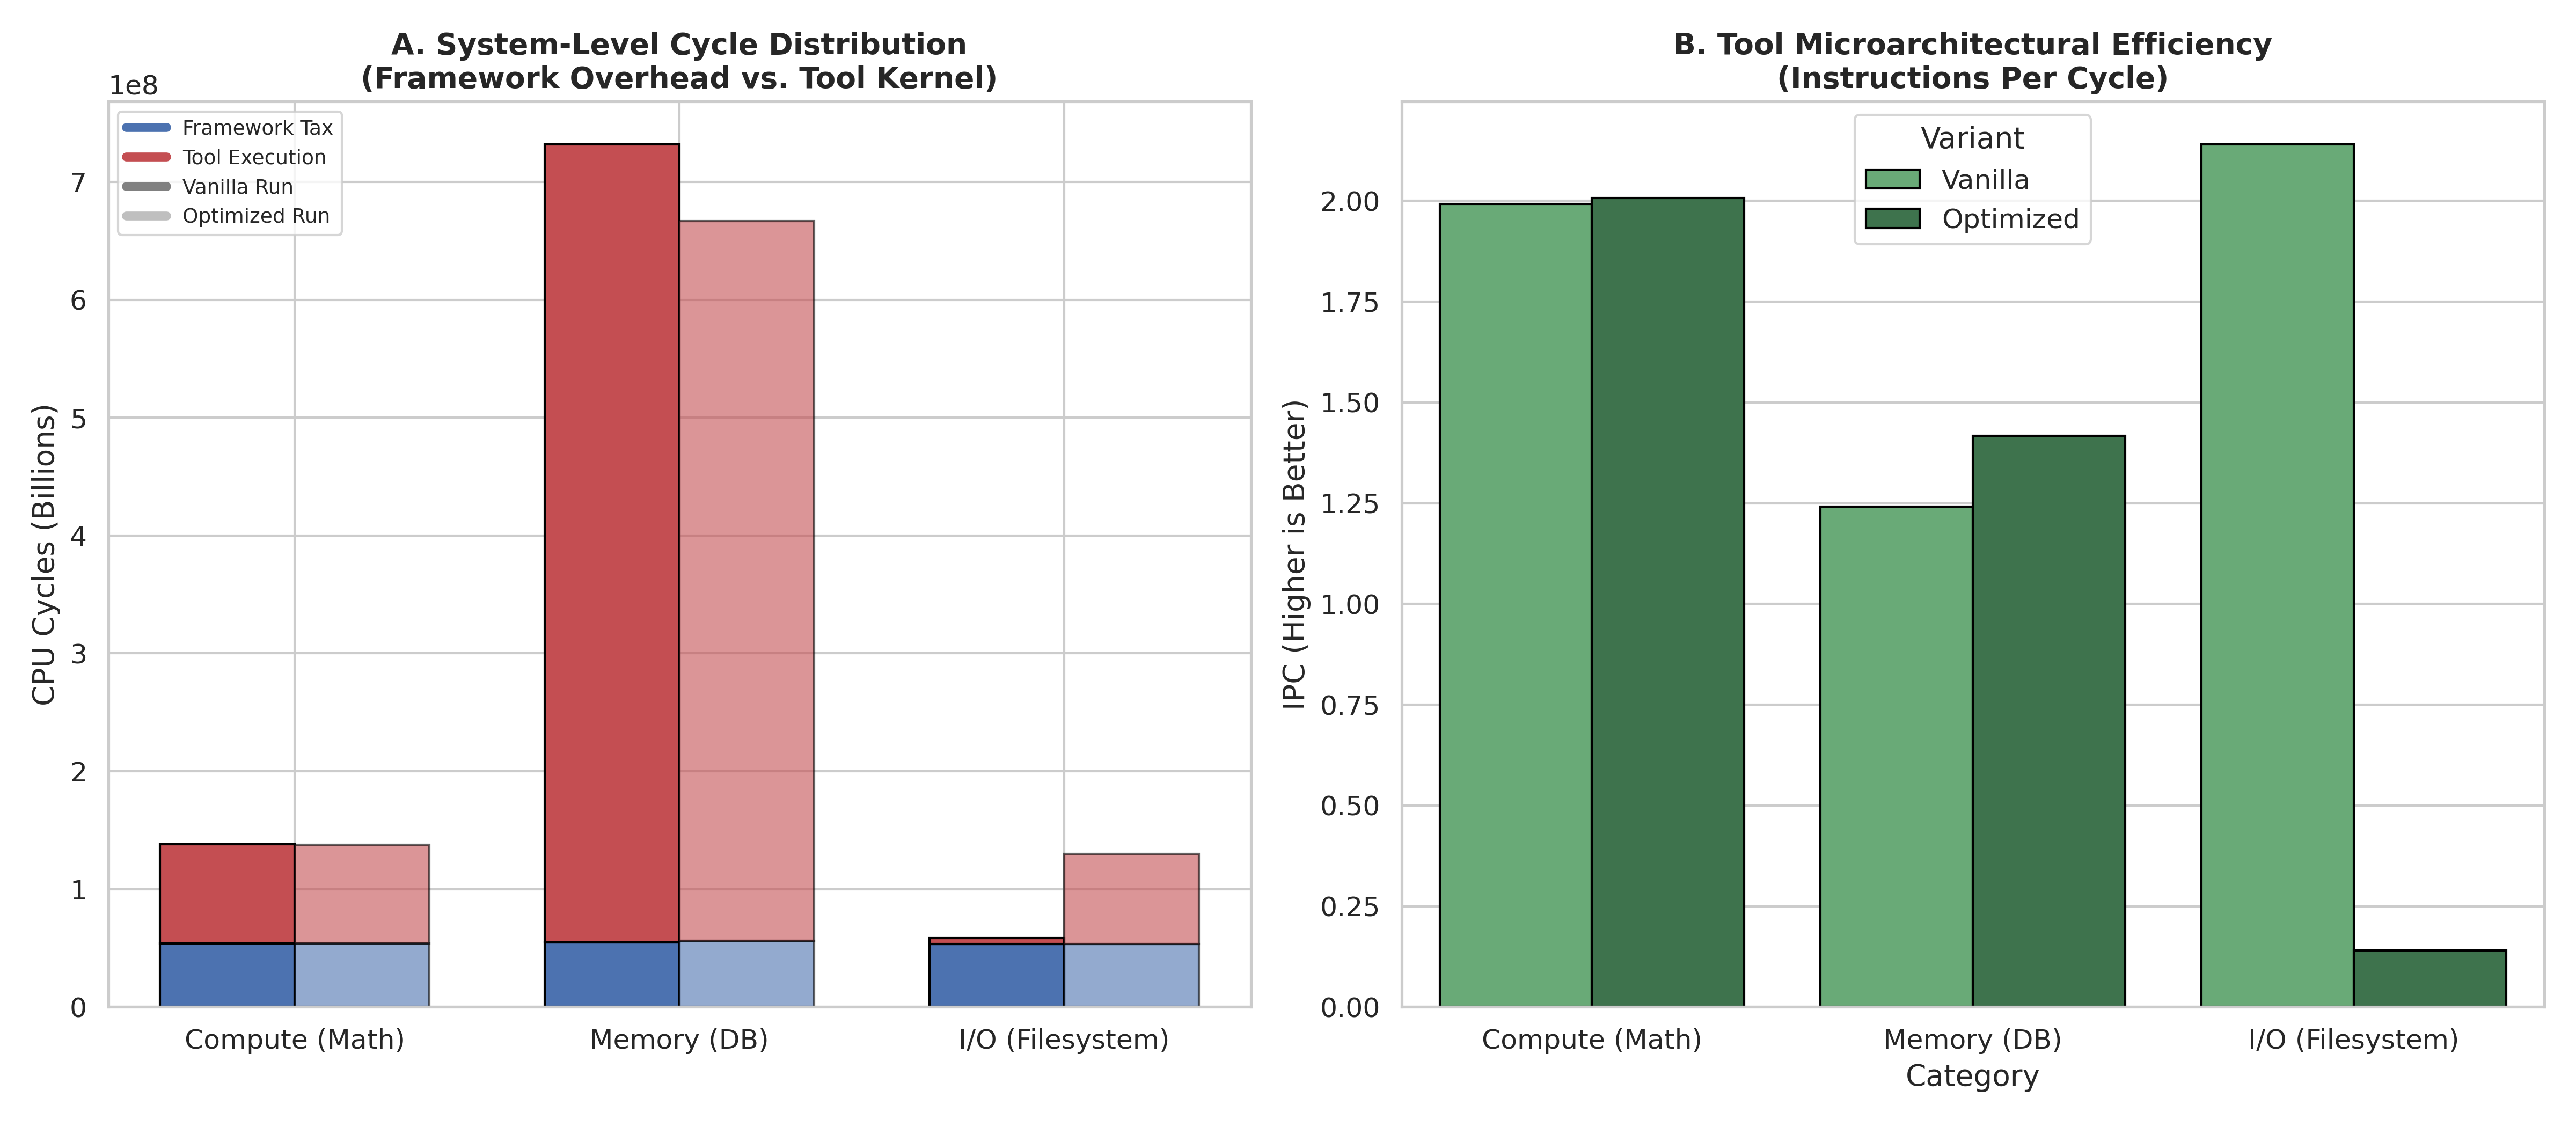
\includegraphics[width=\textwidth]{../results/Final_Research_Comparison.png}
      \end{center}
      \vspace{-0.3em}
      {\scriptsize\textcolor{ash}{Figure 5: System-level cycle distribution across all optimized domains.}}
    \end{column}
    \begin{column}{0.45\textwidth}
      \begin{block}{The Micro Win}
        Software prefetching (\texttt{\_\_builtin\_prefetch}) on the memory-bound DB kernel:
        \begin{itemize}
          \item Kernel IPC \textbf{+14.2\%}
          \item Saved $\sim$\textbf{66\,M} core CPU cycles
        \end{itemize}
      \end{block}
      \vspace{0.3em}
      \begin{alertblock}{The System Reality}
        End-to-end system speedup remained \textbf{below 1\%}.\\[0.3em]
        The massive Python orchestration bloat \textbf{statistically swallows and nullifies} kernel-level microarchitectural victories.
      \end{alertblock}
    \end{column}
  \end{columns}
\end{frame}

% =================================================================
% SLIDE 10: CONCLUSION & FUTURE WORK
% =================================================================
\begin{frame}{Conclusion \& Future Work}
  \begin{tikzpicture}[remember picture, overlay]
    \fill[neonviolet, opacity=0.02] (current page.south east) ++(-2,1) circle (6cm);
  \end{tikzpicture}
  \begin{columns}
    \begin{column}{0.5\textwidth}
      \begin{exampleblock}{The Verdict}
        Current agentic architectures are \textbf{critically crippled} by the orchestration bottleneck. Hardware-software co-design must shift away from optimizing tool-execution kernels and \textbf{aggressively target the orchestration layer itself}.
      \end{exampleblock}
    \end{column}
    \begin{column}{0.5\textwidth}
      \begin{block}{Proposed Solutions}
        \begin{enumerate}
          \item \textcolor{neonmint}{\textbf{Compiled Orchestrators}}\\
                {\small Transitioning to Rust/C++.}
          \item \textcolor{neonviolet}{\textbf{Continuous Batching Engines}}\\
                {\small Adopting vLLM + PagedAttention.}
          \item \textcolor{neonpink}{\textbf{Binary Protocols}}\\
                {\small Replacing JSON with Apache Arrow.}
        \end{enumerate}
      \end{block}
    \end{column}
  \end{columns}
  \vspace{0.6em}
  \begin{center}
    \textcolor{neonmint}{\textbf{Until the orchestration layer is treated as a high-performance data plane,\\
    the promise of agentic AI will remain masked by its own framework.}}
  \end{center}
\end{frame}

% =================================================================
% SLIDE 11: LIVE DEMO & Q&A
% =================================================================
\begin{frame}[plain]
  \begin{tikzpicture}[remember picture, overlay]
    % Abstract decorative geometry
    \draw[neonmint, opacity=0.12, line width=0.4pt] (current page.center) ++(-5,2) -- ++(10,0);
    \draw[neonviolet, opacity=0.08, line width=0.4pt] (current page.center) ++(-3,1.6) -- ++(6,0);
    \draw[neonpink, opacity=0.06, line width=0.4pt] (current page.center) ++(-7,-2) -- ++(14,0);
    \fill[neonmint, opacity=0.03] (current page.south west) ++(3,1) circle (5cm);
    \fill[neonviolet, opacity=0.02] (current page.north east) ++(-2,-2) circle (7cm);
  \end{tikzpicture}
  \begin{center}
    \vspace{1.5em}
    {\Huge\textcolor{bone}{\textbf{Live Demo \& Q\,\&\,A}}}\\
    \vspace{1.5em}
    \textcolor{neonmint}{\rule{4cm}{0.6pt}}\\
    \vspace{1em}
    {\small\textcolor{mist}{Beyond the GPU:}}\\
    {\small\textit{\textcolor{ash}{A Microarchitectural Analysis of LLM Tool-Calling Kernels}}}\\
    \vspace{1.2em}
    {\footnotesize\textcolor{bone}{Terminal 1:} \textcolor{mist}{Run the Orchestrator (\texttt{model\_loader.py})}}\\[0.3em]
    {\footnotesize\textcolor{bone}{Terminal 2:} \textcolor{mist}{Execute the Stress Payloads}}\\
    \vspace{1.2em}
    {\footnotesize\textcolor{ash}{Kunpeng Zhang \quad$\cdot$\quad Fazal Rehman \quad$\cdot$\quad TJ Grewal}}\\
    {\scriptsize\textcolor{ash}{CMPT 450}}\\
    \vspace{0.6em}
    {\scriptsize\textcolor{ash}{\texttt{github.com/AndyZzzZzzZzz/beyond-gpu-kernels}}}
  \end{center}
\end{frame}

\end{document}
